\subsection{Abstract Domains}\label{subsec:abstract-domains}

In the following section we will describe the abstract domains of our value analysis.

\subsubsection{Abstract domain of strings as regular expressions}\label{subsubsec:abstract_domains_strings}
We have chosen regular expressions/languages to represent the abstract domain of the family of SQL string data types.
Regular expressions/languages are chosen instead of more powerful representations because of their decidable nature of inclusion and equality.

Let $REG$ denote the set of regular languages. % and
% \begin{equation*}
%     REG^{\leq n} = \{R \in REG \mid \forall w \in R : |w| \leq n\}.
% \end{equation*}
% In general we do not distinguish between regular expressions and their languages.

The lattice of $(REG, \subseteq, \cup, \cap)$ is a lattice but not a finite one, as the set of regular languages is transfinite and closed under finite union and intersection but not closed under transfinite union and intersection, which makes the lattice not complete.
This is a problem: Essentially, we can not employ the Kleene fixed-point theorem (see \autoref{thm:kleene_finite}) to prove the termination of our analysis.

\subsubsection{Abstract domain of numbers as unions of intervals}\label{subsubsec:abstract_domains_numbers}
We have chosen a finite union of intervals to represent the abstract domain of the family of SQL number data types.
We only consider Integers, but the domain can be extended to the Reals.
$\mathbf{INT}$ is inductivly defined as:
\[
    \inference{\mathscr{I} \text{ is an interval}}{\mathscr{I} \in \mathbf{INT}} \quad
    \inference{\mathscr{I}_1 \in \textbf{INT} & \mathscr{I}_2 \in \textbf{INT}}{\mathscr{I}_1 \cup  \mathscr{I}_2 \in \mathbf{INT}} \quad
    \inference{\mathscr{I}_1 \in \textbf{INT} & \mathscr{I}_2 \in \textbf{INT}}{\mathscr{I}_1 \cap  \mathscr{I}_2 \in \mathbf{INT}}
\]
Let $\mathbf{INT}$ denote the set of union intervals.
The lattice of $(\mathbf{INT}, \sqsubseteq, \sqcup, \sqcap)$ is a lattice but not a finite one, as the set of unions of intervals is transfinite and closed under finite union and intersection but not closed under transfinite union and intersection, which makes the lattice not complete.
We represent such unions of intervals as a set of disjoint intervals; thus, for a set of intervals $\mathscr{I}$:
\begin{equation}
    n \in \gamma(\mathscr{I}) \iff \exists i \in \mathscr{I} : n \in \gamma(i)
\end{equation}
and
\begin{equation}
    \mathscr{I} \sqsubseteq \mathscr{I}' \iff \forall i \in \mathscr{I} : \exists i' \in \mathscr{I}' : i \sqsubseteq i'
\end{equation}
where $\gamma(i)$ is the set of integers in the interval $i$ and $\sqsubseteq$ is the subset relation.
We define the meet and join of unions as follows:
\begin{align}
    \mathscr{I} \sqcup \mathscr{I}' &= m(\mathscr{I} \cup \mathscr{I}') \\
    \text{where } m(\mathscr{I}) &= \begin{cases}
        m(\{ i \sqcup i' | i, i' \in \mathscr{I} \land i \sqcap i' \neq \bot \} \cup \{ i \in \mathscr{I} | \forall i' \in \mathscr{I} : i \sqcap i' = \bot \}) & \text{if } \exists i, i' \in \mathscr{I}: i \sqcap i' \neq \bot \\
        \mathscr{I} & \text{otherwise}
    \end{cases} \\
    \mathscr{I} \sqcap \mathscr{I}' &= \{i \sqcap i' \mid i \in \mathscr{I} \land i' \in \mathscr{I}'\}
\end{align}

This intuitively models intersection and union of the underlying sets, that is $\gamma(\mathscr{I} \sqcup \mathscr{I}') = \gamma(\mathscr{I}) \cup \gamma(\mathscr{I}')$ (analogous for $\sqcap$, $\cap$), and also $\mathscr{I} \sqsubseteq \mathscr{I}' \iff \gamma(\mathscr{I}) \subseteq \gamma(\mathscr{I}')$.

This representation of numbers has the same issue as regular expressions: it is not finite and thus not complete, which makes it impossible to use the Kleene fixed-point theorem (see \autoref{thm:kleene_finite}) to prove the termination of our analysis.

\subsubsection{Single and List values}

We would like to distinguish between single values and lists of values, thus we define algebraic type:
\begin{align}
    \mathsf{Val} \; A = \{ \mathsf{Single} \; a \mid a \in A \} \cup \{ \mathsf{List} \; A' \mid A' \subseteq A \}
\end{align}
We define the following operations on the algebraic type:
\begin{align}
    \mathsf{Single} \; s &\sqsubseteq \mathsf{List} \; S \quad
    \text{iff} \; s \in S \\
    \mathsf{Single} \; s_1 &\sqsubseteq \mathsf{Single} \; s_2 \quad
    \text{iff} \; s_1 \sqsubseteq s_2 \\
    \mathsf{List} \; S &\not\sqsubseteq \mathsf{Single} \; s\\
    \mathsf{List} \; S_1 &\sqsubseteq \mathsf{List} \; S_2 \quad
    \text{iff} \; \forall s_1 \in S_1, \; \exists s_2 \in S_2: \; s_1 \sqsubseteq s_2\\
    \mathsf{Single} \; s \sqcup \mathsf{List} \; S &= \mathsf{List} \; (S\sqcup\left\{ s \right\})\\
    \mathsf{Single} \; s_1 \sqcup \mathsf{Single} \; s_2 &= \mathsf{Single} \; (s \sqcup s )\\
    \mathsf{List} \; S_1 \sqcup \mathsf{List} \; S_2 &= \mathsf{List} \; (S_1 \sqcup S_2)\\
    \mathsf{Single} \; s \sqcap \mathsf{List} \; S &= \mathsf{Single} \; s\\
    \mathsf{List} \; S_1 \sqcap \mathsf{List} \; S_2 &= \mathsf{List} \; (S_1 \sqcap S_2)\\
    \mathsf{Single} \; s_1 \sqcap \mathsf{Single} \; s_2 &= \mathsf{Single} \; (s_1 \sqcap s_2)
\end{align}

\subsubsection{Cover lattice}
To resolve the issue presented above we introduce the notion of a cover lattice, but first we need to define a collectively disjoint top-cover and a cover lattice.

\begin{definition}
    A finite non-empty subset $X \subseteq S$ of a lattice $(S, \subseteq, \cup, \cap)$ is called a collectively top-cover of $S$ whenever $\bigcup X = \top$.
\end{definition}

\begin{definition}\label{def:coverlattice}
Given a collectively top-cover $X$ of a lattice $(S, \subseteq, \cup, \cap)$.
A cover lattice of $S$ in respect to $X$ denoted $\clattice{X}{S}$ is the minimum set where,
For $X$ and $S$:
    $\inference{x \in X}{x \in C_X(S)} \quad
    \inference{x_1 \in C_X(S) & x_2 \in C_X(S)}{x_1 \cup  x_2 \in C_X(S)} \quad
    \inference{x_1 \in C_X(S) & x_2 \in C_X(S)}{x_1 \cap  x_2 \in C_X(S)}$
\end{definition}

Now we can define the cover lattice of the regular languages and the integers.
This gives rise to the following theorem:

\begin{restatable}{theorem}{partition}\label{thm:partition}
For a non-complete lattice $(S, \subseteq, \cup, \cap)$ and collectively top-cover $X$ of $S$, the cover lattice $(\clattice{X}{S}, \subseteq, \cup, \cap)$ is a finite and complete lattice.
\end{restatable}

And the following lemmas immediately follow:

\begin{lemma}
    If $\mathcal{R}$ is a collectively top-cover of $(REG, \subseteq, \cup, \cap)$ then $(\clattice{\mathcal{R}}{REG}, \subseteq, \cup, \cap)$ is a complete lattice.
\end{lemma}

\begin{lemma}
    If $X$ is a collectively top-cover of $(\mathscr{Z}, \subseteq, \cup, \cap)$ then $(\clattice{X}{\mathscr{Z}}, \subseteq, \cup, \cap)$ is a complete lattice.
\end{lemma}

\begin{definition}
    We define $\cdot \into C_X(S):S\rightarrow C_X(S)$ to be the function mapping $s\in S$ to the least element in $C_X(S)$ containing it, that is $s \into C_X(S)=\bigsqcap\{s'\in C_X(S)|s\sqsubseteq s'\}$
    \\

    We define $\cdot \into C_X(S):\mathcal{P}(S)\rightarrow \mathcal{P}(C_X(S))$ to be the function that maps the powerset of the lattice elements to the powerset of the cover lattice elements.
    We use $H \into C_X (S) = \{h \into C_X (S) \mid h \in H\}$ to show how a set of elements is mapped to the cover lattice.
\end{definition}

\begin{definition}
    We define $\circ \into C_\mathcal{X}(\mathcal{S}): \bigtimes_{i = 1}^{n} S_i \rightarrow \bigtimes_{i = 1}^{n} C_{X_i}(S_i)$ to be the function that takes a tuple and inserts each element of the tuple correctly into its given cover lattice.
    We use $(h_1, h_2 \dots h_n)\into C_{\mathcal{X}}(\mathcal{S})=(h_1 \into C_{X_1}(S_1), h_2\into C_{X_2}(S_2), \dots, h_n \into C_{X_n}(S_n))$
    $\mathcal{X}=(X_1, X_2, \dots, X_n)$
    $\mathcal{S}=(S_1, S_2, \dots, S_n)$ to show the type of the function and what $\mathcal{X}$ and $\mathcal{S}$ are.
\end{definition}

\begin{definition}
    We define $\circ \into C_X(S): \ \mathsf{Val} \ S \rightarrow \mathsf{Val} \ C_X(S)$ to be the function that takes some value and inserts it ito its cover lattice. \\
    For single elements we use $(\mathsf{Single} \ h) \into C_x(S) = \mathsf{Single}(h\into C_x(S))$ where $x \in (\mathsf{Single} \ x') \ \text{iff} \ x = x'$ \\
    And for a list of elements, we use $(\mathsf{List} \ H) \into C_x(S)=\mathsf{List}(H\into C_x(S))$ where $x \in (\mathsf{List} \ X) \ \text{iff} \ x \in X$ \\
\end{definition}

\begin{example}
    \autoref{fig:tikz-reg-partition} illustrates a simple lattice cover of the regular languages.
    The regular language $R$ is represented by the gray circle and its complement $\overline{R}$ is represented by the white circle.
    The union of the two regular language represent the entire regular language $\Sigma^*$ and their intersection is the empty set $\emptyset$.

    \autoref{fig:tikz-reg-partition-lattice} illustrates the cover lattice induced by the lattice cover.
    The top element $\top$ is the entire regular language $\Sigma^*$ and the bottom element $\bot$ is the empty set $\emptyset$.
\end{example}

% Tikzfigures
\begin{figure}
    \center
    \resizebox{7.5cm}{!}{
    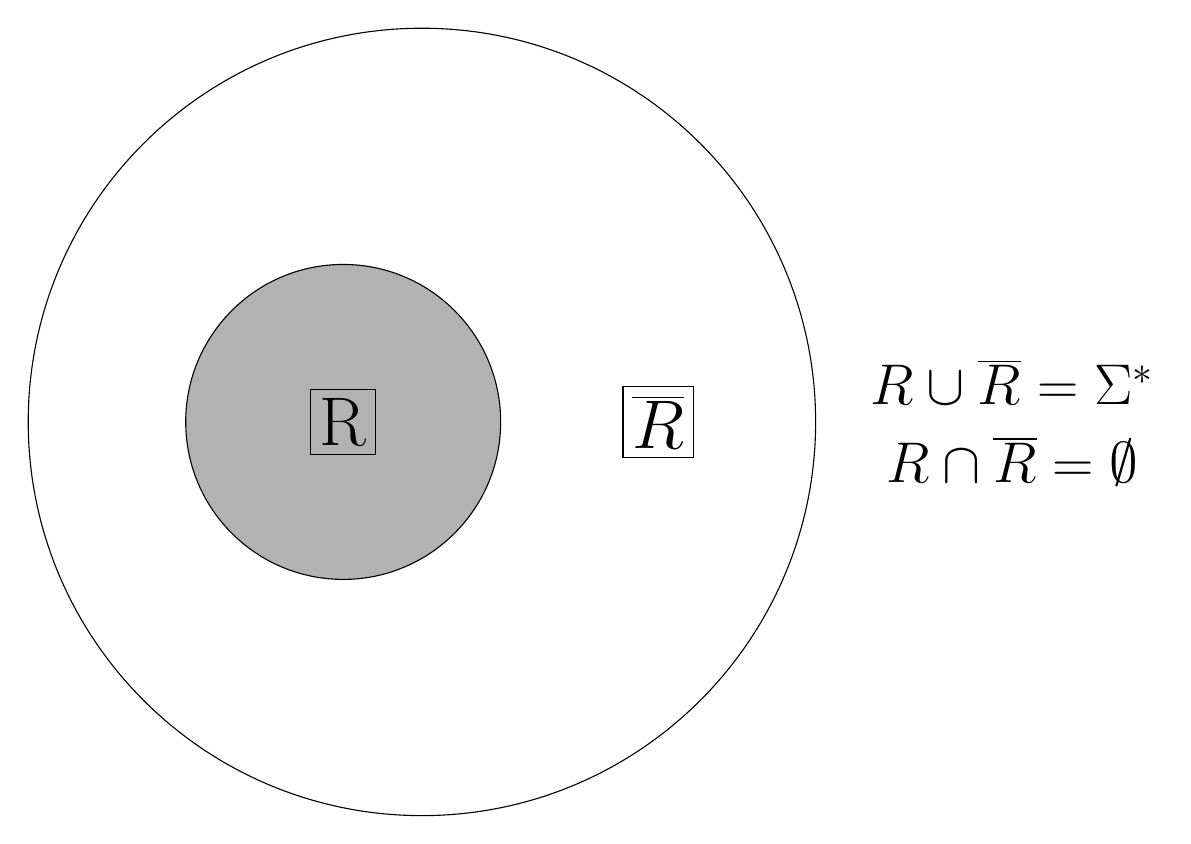
\begin{tikzpicture}
    \filldraw[fill=white, draw=black] (2,2) circle (5cm);
    \node [draw] at (5,2) {\Huge$\overline{R}$};
    \filldraw[fill=gray!60, draw=black] (1,2) circle (2cm);
    \node [draw] at (1,2) {\Huge R};
    \node at (9.5, 2.5) {\huge $R \cup \overline{R} = \Sigma^*$};
    \node at (9.5, 1.5) {\huge $R \cap \overline{R} = \emptyset$};
\end{tikzpicture}}
    \caption{Regular language partition}
    \label{fig:tikz-reg-partition}
\end{figure}

\begin{figure}[!htb]
    \center
    \resizebox{6.5cm}{!}{
    \begin{tikzpicture}[scale = 0.5]
    \usetikzlibrary{calc}
    \node (a) [state] {\Huge$R \cup \overline{R} = \top = \Sigma^*$};
    \node (b1) [state, shift={($(a.south)+(3cm, -2.5cm)$)}] {\Huge $R$};
    \node (b2) [state, shift={($(a.south)+(-3cm, -2.5cm)$)}]{\Huge $\overline{R}$};
    \node (c) [state, shift= {($(a.south) + (0cm, -5.5cm)$)}] {\Huge $R \cap \overline{R} = \bot = \emptyset$};
    \draw (a) to (b1);
    \draw (a) to (b2);
    \draw (b1) to (c);
    \draw (b2) to (c);
\end{tikzpicture}}
    \caption{Regular language partition as a lattice}
    \label{fig:tikz-reg-partition-lattice}
\end{figure}

\subsubsection{Abstract domain of tables}\label{subsubsec:abstract_domain_of_tables}

We consider a table $t$ as function from the domain of possible tuples in the table $\mathbb{T}$ to the codomain of natural numbers including $0$, $\mathbb{N}$:
\begin{equation}
    t : \mathbb{T} \rightarrow \mathbb{N}.
\end{equation}
The function $t$ describe the number of a given tuple in a table.
We can then consider abstraction over the table $t$ by abstracting either the domain or codomain
This gives rise to a taxonomy of abstract domains of tables shown in \autoref{tab:taxonomy_of_abstract_domain_of_tables}.
In \autoref{tab:taxonomy_of_abstract_domain_of_tables} $\mathbb{T}^\#$ let denote an abstract domain of the set of possible tuples $\mathbb{T}$, such that it forms a finite lattice $(\mathbb{T}^\#, \sqsubseteq, \sqcap, \sqcup)$ (and analogous for $\mathbb{N}$).

\begin{table}
    \caption{Taxonomy of abstract domains of tables}
    \centering
    \begin{tabular}{c|l|c}
    Name & Function & Supported \\
    \hline
    \hline
        Bag of tuples & $\mathbb{T} \rightarrow \mathbb{N}$ & \\
        Abstract bag of tuples & $\mathbb{T} \rightarrow \mathbb{N}^\#$ & \\
        Set of tuples & $\mathbb{T} \rightarrow 2$ & \\
        Bag of abstract tuples & $\mathbb{T}^\# \rightarrow \mathbb{N}$ & \\
        Abstract bag of abstract tuples & $\mathbb{T}^\# \rightarrow \mathbb{N}^\#$ & \checkmark \\
        Set of abstract tuples & $\mathbb{T}^\# \rightarrow \{0, some\}$ & \checkmark \\
        Abstract tuple & $\{\cdot\} \rightarrow \mathbb{T}^\#$ & \checkmark \\
    \end{tabular}
    \label{tab:taxonomy_of_abstract_domain_of_tables}
\end{table}

We will only consider abstract bags of abstract tuples, sets of abstract tuples and abstract tuples because of their finite nature.
It should be clear that sets of abstract tuples are just a special case of abstract bags of abstract tuples.
Naturally, these maps all form map lattices.
